\section*{\textbf{6 - Classifying x-ray bursts} \hrule} 



\subsection*{\textbf{Question 6}}
\begin{quote}

\textbf{Problem}
\begin{quote}
Use logistic regression to make a model of the data, suing a binary classification for short or long GRBs. Explain which properties your model uses to prediced whether a GRB is short or long, and how you handle missing data. Plot a histogram of the class (0 or 1) of GRB and overplot the actual class based on the value of $T_{90}$.
\end{quote}

\textbf{Solution} 
\begin{quote}


The data is before training the model pre-processed as follows. The first stap consists of removing all rows with missing $T_{90}$ (this only consists of two rows). Next, the columns with  logarithmic values are taken to the power of an exponent. Finally the values of $-1$ in the non logarithmic columns and the values of $e^{-1}$ in the logarithmic columns are replaced with 0. The reason that the columns with logarithmic values where first taken to the exponent is because directly replacing -1.0 in such a column with 0 is equivalent to creating your own data. (i.e if $\ln(M_{*}/M_{\odot}) = 0$, then we would have created data that implies that $M_{*} = M_{\odot}$). 
\\
The columns that where chosen for training  consist of the redshift, the star formation rate and the log of the mass ratio. These columns where selected based on a scatter plot made with seaborn in which all columns where plotted against each other. The code for this is not included\footnote{I did not had enough time to recreate the plot without seaborn before the deadline.}. 
\\
With these columns an accuracy of 78 \% was obtained (see page 80). This value is unfortunately the base line that needs to be broken, as in the final dataset 78\% of all entries are long GRBS. The model is thus returning '1' for each entry. Attempts to use different combinations of columns always resulted in the same accuracy. The code that creates the histogram and the code for the logistic regression can be found below.  

\end{quote}

\textbf{Code - Plot}
\begin{quote}
The code that creates the plots.
%The code that creates the slices, cell 0 and cell 4 in a 3D grid of size 16.
\lstinputlisting{./Code/assigment_6.py}
\end{quote}

\textbf{Code - Logistic regression}
\begin{quote}
The code for logistic regression.
%The code that creates the slices, cell 0 and cell 4 in a 3D grid of size 16.
\lstinputlisting{./Code/mathlib/LogisticRegression.py}
\end{quote}
\newpage

\textbf{Text - Output} \\

The accuracy obtained by the model.
\begin{quote}
\lstinputlisting{./Output/assigment6_out.txt}
\end{quote}

\textbf{Plots- Histogram}
\begin{figure}[!hb]
\centering
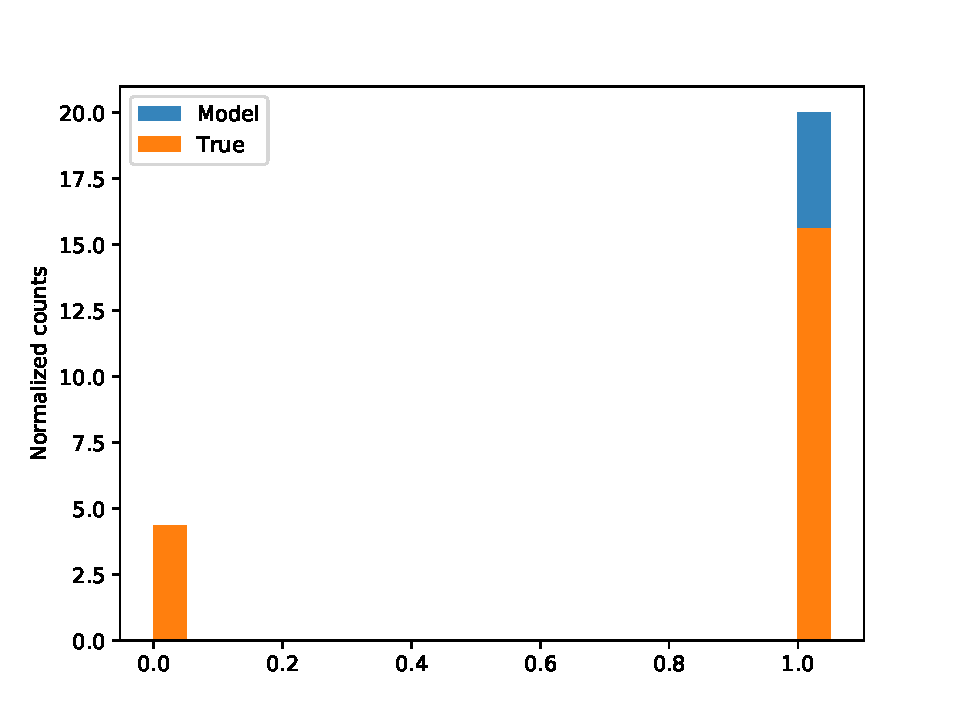
\includegraphics[width=14cm, height=7.5cm]{./Plots/6a_hist.pdf}
\caption{The created histogram for the prediction made by the model and the true labels. It can be seen here that the model always returns '1'. }
\end{figure}

\begin{quote} 


\end{quote}
\end{quote}







